\documentclass{standalone}
\usepackage{tikz}
\usetikzlibrary{patterns, positioning}
\usepackage[sfdefault]{ClearSans} %% option 'sfdefault' activates Clear Sans as the default text font
\usepackage[T1]{fontenc}

\begin{document}
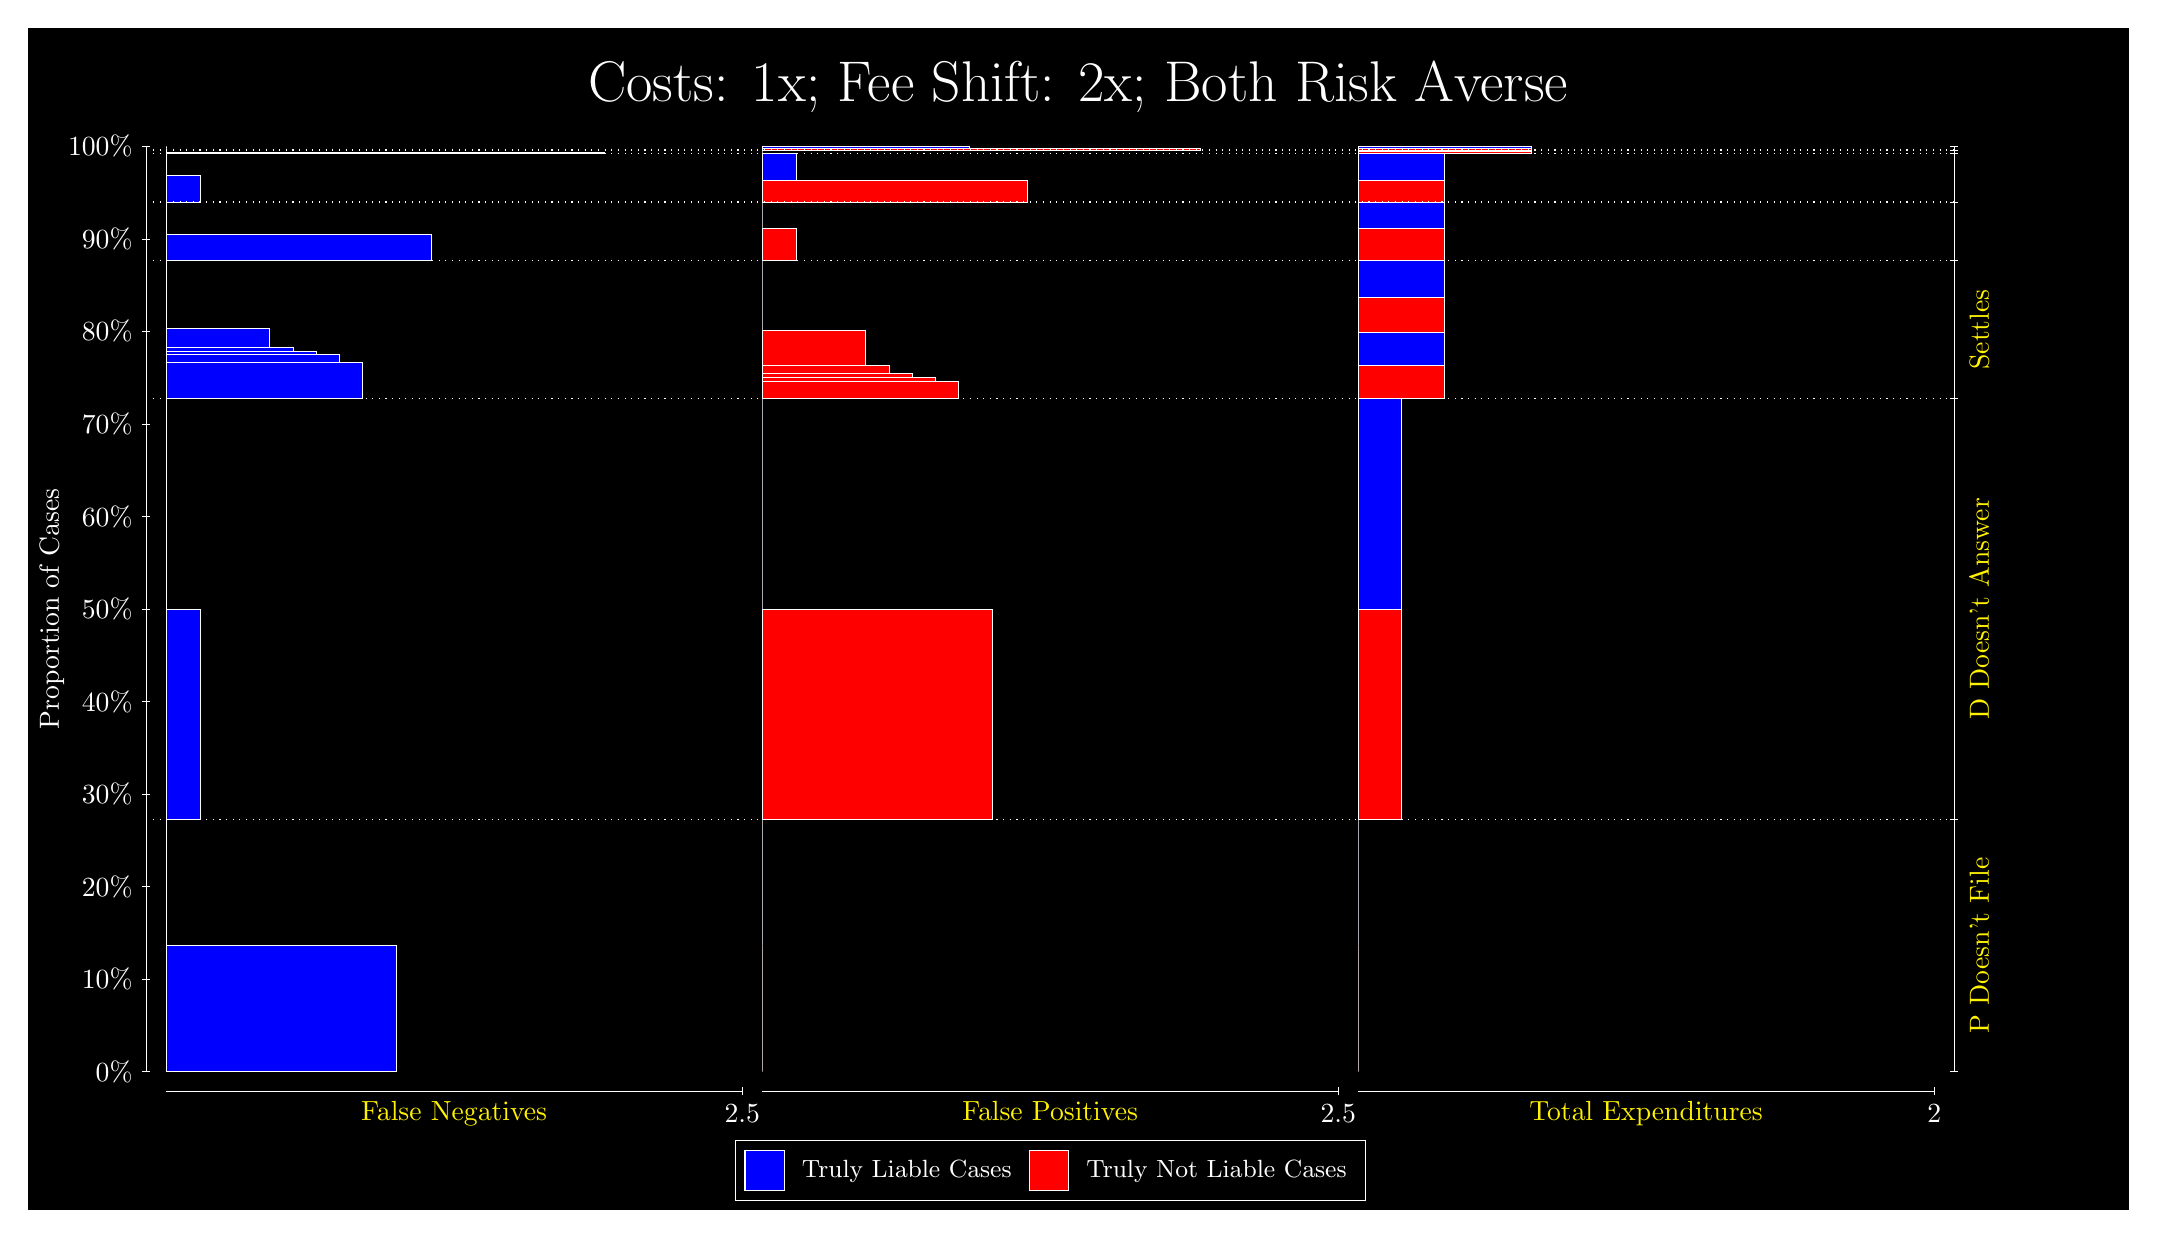
\begin{tikzpicture}
\draw[fill=black] (0,0) rectangle (26.667,15);
\draw[text=white] (0,13.5) rectangle (26.667,15) node[midway] {\huge Costs: 1x; Fee Shift: 2x; Both Risk Averse};
\draw[white, very thin] (1.5,1.75) -- (1.5,13.5);
\node[rotate=90, text=white, anchor=center] at (0.3, 7.625) {Proportion of Cases};
\draw[white, very thin] (1.45,1.75) -- (1.55,1.75);
\node[text=white, anchor=east] at (1.45, 1.75) {0\%};
\draw[white, very thin] (1.45,2.925) -- (1.55,2.925);
\node[text=white, anchor=east] at (1.45, 2.925) {10\%};
\draw[white, very thin] (1.45,4.1) -- (1.55,4.1);
\node[text=white, anchor=east] at (1.45, 4.1) {20\%};
\draw[white, very thin] (1.45,5.275) -- (1.55,5.275);
\node[text=white, anchor=east] at (1.45, 5.275) {30\%};
\draw[white, very thin] (1.45,6.45) -- (1.55,6.45);
\node[text=white, anchor=east] at (1.45, 6.45) {40\%};
\draw[white, very thin] (1.45,7.625) -- (1.55,7.625);
\node[text=white, anchor=east] at (1.45, 7.625) {50\%};
\draw[white, very thin] (1.45,8.8) -- (1.55,8.8);
\node[text=white, anchor=east] at (1.45, 8.8) {60\%};
\draw[white, very thin] (1.45,9.975) -- (1.55,9.975);
\node[text=white, anchor=east] at (1.45, 9.975) {70\%};
\draw[white, very thin] (1.45,11.15) -- (1.55,11.15);
\node[text=white, anchor=east] at (1.45, 11.15) {80\%};
\draw[white, very thin] (1.45,12.325) -- (1.55,12.325);
\node[text=white, anchor=east] at (1.45, 12.325) {90\%};
\draw[white, very thin] (1.45,13.5) -- (1.55,13.5);
\node[text=white, anchor=east] at (1.45, 13.5) {100\%};

\draw[white, very thin] (24.457,1.75) -- (24.457,13.5);
\draw[white, very thin] (24.407,1.75) -- (24.507,1.75);
\node[anchor=west] at (24.407, 1.75) {};
\draw[white, very thin] (24.407,4.9545) -- (24.507,4.9545);
\node[anchor=west] at (24.407, 4.9545) {};
\draw[white, very thin] (24.407,10.295) -- (24.507,10.295);
\node[anchor=west] at (24.407, 10.295) {};
\draw[white, very thin] (24.407,12.051) -- (24.507,12.051);
\node[anchor=west] at (24.407, 12.051) {};
\draw[white, very thin] (24.407,12.793) -- (24.507,12.793);
\node[anchor=west] at (24.407, 12.793) {};
\draw[white, very thin] (24.407,13.406) -- (24.507,13.406);
\node[anchor=west] at (24.407, 13.406) {};
\draw[white, very thin] (24.407,13.453) -- (24.507,13.453);
\node[anchor=west] at (24.407, 13.453) {};
\draw[white, very thin] (24.407,13.5) -- (24.507,13.5);
\node[anchor=west] at (24.407, 13.5) {};

\draw[white, very thin, fill=blue] (1.75,1.75) rectangle (4.6775,3.3523);
\draw[white, very thin, fill=red] (1.75,3.3523) rectangle (1.75,4.9545);
\draw[white, very thin, fill=blue] (1.75,4.9545) rectangle (2.1891,7.625);
\draw[white, very thin, fill=red] (1.75,7.625) rectangle (1.75,10.295);
\draw[white, very thin, fill=blue] (1.75,10.295) rectangle (4.2384,10.76);
\draw[white, very thin, fill=blue] (1.75,10.76) rectangle (3.9457,10.864);
\draw[white, very thin, fill=blue] (1.75,10.864) rectangle (3.6529,10.903);
\draw[white, very thin, fill=blue] (1.75,10.903) rectangle (3.3602,10.95);
\draw[white, very thin, fill=blue] (1.75,10.95) rectangle (3.0674,11.184);
\draw[white, very thin, fill=red] (1.75,11.184) rectangle (1.75,12.051);
\draw[white, very thin, fill=blue] (1.75,12.051) rectangle (5.1167,12.38);
\draw[white, very thin, fill=red] (1.75,12.38) rectangle (1.75,12.793);
\draw[white, very thin, fill=blue] (1.75,12.793) rectangle (2.1891,13.13);
\draw[white, very thin, fill=red] (1.75,13.13) rectangle (1.75,13.406);
\draw[white, very thin, fill=blue] (1.75,13.406) rectangle (7.3123,13.428);
\draw[white, very thin, fill=red] (1.75,13.428) rectangle (1.75,13.453);
\draw[white, very thin, fill=red] (1.75,13.453) rectangle (1.75,13.474);
\draw[white, very thin, fill=blue] (1.75,13.474) rectangle (1.75,13.5);
\draw[white, very thin, fill=red] (9.3189,1.75) rectangle (9.3189,3.3523);
\draw[white, very thin, fill=blue] (9.3189,3.3523) rectangle (9.3189,4.9545);
\draw[white, very thin, fill=red] (9.3189,4.9545) rectangle (12.246,7.625);
\draw[white, very thin, fill=blue] (9.3189,7.625) rectangle (9.3189,10.295);
\draw[white, very thin, fill=red] (9.3189,10.295) rectangle (11.807,10.516);
\draw[white, very thin, fill=red] (9.3189,10.516) rectangle (11.515,10.572);
\draw[white, very thin, fill=red] (9.3189,10.572) rectangle (11.222,10.616);
\draw[white, very thin, fill=red] (9.3189,10.616) rectangle (10.929,10.717);
\draw[white, very thin, fill=red] (9.3189,10.717) rectangle (10.636,11.162);
\draw[white, very thin, fill=blue] (9.3189,11.162) rectangle (9.3189,12.051);
\draw[white, very thin, fill=red] (9.3189,12.051) rectangle (9.758,12.464);
\draw[white, very thin, fill=blue] (9.3189,12.464) rectangle (9.3189,12.793);
\draw[white, very thin, fill=red] (9.3189,12.793) rectangle (12.686,13.069);
\draw[white, very thin, fill=blue] (9.3189,13.069) rectangle (9.758,13.406);
\draw[white, very thin, fill=red] (9.3189,13.406) rectangle (9.3189,13.431);
\draw[white, very thin, fill=blue] (9.3189,13.431) rectangle (9.3189,13.453);
\draw[white, very thin, fill=red] (9.3189,13.453) rectangle (14.881,13.474);
\draw[white, very thin, fill=blue] (9.3189,13.474) rectangle (11.954,13.5);
\draw[white, very thin, fill=red] (16.888,1.75) rectangle (16.888,3.3523);
\draw[white, very thin, fill=blue] (16.888,3.3523) rectangle (16.888,4.9545);
\draw[white, very thin, fill=red] (16.888,4.9545) rectangle (17.437,7.625);
\draw[white, very thin, fill=blue] (16.888,7.625) rectangle (17.437,10.295);
\draw[white, very thin, fill=red] (16.888,10.295) rectangle (17.986,10.717);
\draw[white, very thin, fill=blue] (16.888,10.717) rectangle (17.986,11.141);
\draw[white, very thin, fill=red] (16.888,11.141) rectangle (17.986,11.587);
\draw[white, very thin, fill=blue] (16.888,11.587) rectangle (17.986,12.051);
\draw[white, very thin, fill=red] (16.888,12.051) rectangle (17.986,12.464);
\draw[white, very thin, fill=blue] (16.888,12.464) rectangle (17.986,12.793);
\draw[white, very thin, fill=red] (16.888,12.793) rectangle (17.986,13.069);
\draw[white, very thin, fill=blue] (16.888,13.069) rectangle (17.986,13.406);
\draw[white, very thin, fill=red] (16.888,13.406) rectangle (19.083,13.431);
\draw[white, very thin, fill=blue] (16.888,13.431) rectangle (19.083,13.453);
\draw[white, very thin, fill=red] (16.888,13.453) rectangle (19.083,13.474);
\draw[white, very thin, fill=blue] (16.888,13.474) rectangle (19.083,13.5);
\draw[white, dotted] (1.5,4.9545) -- (24.457,4.9545);
\draw[white, dotted] (1.5,10.295) -- (24.457,10.295);
\draw[white, dotted] (1.5,12.051) -- (24.457,12.051);
\draw[white, dotted] (1.5,12.793) -- (24.457,12.793);
\draw[white, dotted] (1.5,13.406) -- (24.457,13.406);
\draw[white, dotted] (1.5,13.453) -- (24.457,13.453);
\draw[white, very thin] (1.75,1.5) -- (9.0689,1.5);
\node[text=yellow, anchor=north] at (5.4094, 1.5) {False Negatives};
\draw[white, very thin] (9.0689,1.45) -- (9.0689,1.55);
\node[text=white, anchor=north] at (9.0689, 1.45) {2.5};

\draw[white, very thin] (9.3189,1.5) -- (16.638,1.5);
\node[text=yellow, anchor=north] at (12.978, 1.5) {False Positives};
\draw[white, very thin] (16.638,1.45) -- (16.638,1.55);
\node[text=white, anchor=north] at (16.638, 1.45) {2.5};

\draw[white, very thin] (16.888,1.5) -- (24.207,1.5);
\node[text=yellow, anchor=north] at (20.547, 1.5) {Total Expenditures};
\draw[white, very thin] (24.207,1.45) -- (24.207,1.55);
\node[text=white, anchor=north] at (24.207, 1.45) {2};

\node[text=yellow, centered, rotate=90] at (24.777, 3.3523) {P Doesn't File};
\node[text=yellow, centered, rotate=90] at (24.777, 7.625) {D Doesn't Answer};
\node[text=yellow, centered, rotate=90] at (24.777, 11.173) {Settles};





\draw (12.978300999999998,1.5) node[draw=none] (baseCoordinate) {};
\begin{scope}[align=center]
        \matrix[scale=0.5, draw=white, below=0.5cm of baseCoordinate, nodes={draw}, column sep=0.1cm]{
            \node[rectangle, draw, minimum width=0.5cm, minimum height=0.5cm, fill=blue] {}; &
            \node[draw=none, font=\small, text=white] (B) {Truly Liable Cases}; &
            \node[rectangle, draw, minimum width=0.5cm, minimum height=0.5cm, fill=red] {}; &
            \node[draw=none, font=\small, text=white] (B) {Truly Not Liable Cases}; \\
            };
\end{scope}

\end{tikzpicture}
\end{document}